% Options for packages loaded elsewhere
\PassOptionsToPackage{unicode}{hyperref}
\PassOptionsToPackage{hyphens}{url}
%
\documentclass[
]{book}
\usepackage{amsmath,amssymb}
\usepackage{iftex}
\ifPDFTeX
  \usepackage[T1]{fontenc}
  \usepackage[utf8]{inputenc}
  \usepackage{textcomp} % provide euro and other symbols
\else % if luatex or xetex
  \usepackage{unicode-math} % this also loads fontspec
  \defaultfontfeatures{Scale=MatchLowercase}
  \defaultfontfeatures[\rmfamily]{Ligatures=TeX,Scale=1}
\fi
\usepackage{lmodern}
\ifPDFTeX\else
  % xetex/luatex font selection
\fi
% Use upquote if available, for straight quotes in verbatim environments
\IfFileExists{upquote.sty}{\usepackage{upquote}}{}
\IfFileExists{microtype.sty}{% use microtype if available
  \usepackage[]{microtype}
  \UseMicrotypeSet[protrusion]{basicmath} % disable protrusion for tt fonts
}{}
\makeatletter
\@ifundefined{KOMAClassName}{% if non-KOMA class
  \IfFileExists{parskip.sty}{%
    \usepackage{parskip}
  }{% else
    \setlength{\parindent}{0pt}
    \setlength{\parskip}{6pt plus 2pt minus 1pt}}
}{% if KOMA class
  \KOMAoptions{parskip=half}}
\makeatother
\usepackage{xcolor}
\usepackage{graphicx}
\makeatletter
\newsavebox\pandoc@box
\newcommand*\pandocbounded[1]{% scales image to fit in text height/width
  \sbox\pandoc@box{#1}%
  \Gscale@div\@tempa{\textheight}{\dimexpr\ht\pandoc@box+\dp\pandoc@box\relax}%
  \Gscale@div\@tempb{\linewidth}{\wd\pandoc@box}%
  \ifdim\@tempb\p@<\@tempa\p@\let\@tempa\@tempb\fi% select the smaller of both
  \ifdim\@tempa\p@<\p@\scalebox{\@tempa}{\usebox\pandoc@box}%
  \else\usebox{\pandoc@box}%
  \fi%
}
% Set default figure placement to htbp
\def\fps@figure{htbp}
\makeatother
\setlength{\emergencystretch}{3em} % prevent overfull lines
\providecommand{\tightlist}{%
  \setlength{\itemsep}{0pt}\setlength{\parskip}{0pt}}
\setcounter{secnumdepth}{5}
\ifLuaTeX
\usepackage[bidi=basic]{babel}
\else
\usepackage[bidi=default]{babel}
\fi
\babelprovide[main,import]{italian}
% get rid of language-specific shorthands (see #6817):
\let\LanguageShortHands\languageshorthands
\def\languageshorthands#1{}
          \usepackage{cancel}
          \usepackage{tikz}
          \usepackage[version=4]{mhchem}
          \usepackage{circuitikz}
          \usepackage{steinmetz}
          \usepackage{derivative}
          \usepackage{tabularray}
          \usepackage{mathtools}
          \usepackage{siunitx}
          \usepackage{tcolorbox}
          \usepackage{geometry}
          \usepackage{array}
          \usepackage{caption}
          \usepackage{sectsty}
          \usepackage{hhline}
              \geometry{
                  a4paper,
                  total={170mm,257mm},
                  left=20mm,
                  top=20mm,
              }
          \tcbuselibrary{most}
          \newtcolorbox[auto counter,number within=section]{mybox}[1]{colback=red!5!white, colframe=red!75!black,
          fonttitle=\bfseries, title={#1}}
\usepackage{bookmark}
\IfFileExists{xurl.sty}{\usepackage{xurl}}{} % add URL line breaks if available
\urlstyle{same}
\hypersetup{
  pdftitle={Appunti Elettronica generale},
  pdfauthor={Leonardo Toccafondi},
  pdflang={it},
  pdfsubject={Elettronica},
  hidelinks,
  pdfcreator={LaTeX via pandoc}}

\title{Appunti Elettronica generale}
\author{Leonardo Toccafondi}
\date{2024-04-12}

\begin{document}
\frontmatter
\maketitle

{
\setcounter{tocdepth}{2}
\tableofcontents
}
\mainmatter
\chapter{Dispositivi elettronici}\label{dispositivi-elettronici}

\section{Semiconduttori}\label{semiconduttori}

I semiconduttori sono i materiali con cui sono composti i circuiti
integrati. Sono, come suggerisce il nome, materiali in cui il flusso di
corrente \emph{non è libero} (non è un conduttore), ma è
\textbf{presente} (non è un'isolante).

In particolare, conducono in particolari situazioni. Quali sono però i
materiali con queste condizioni?

\begin{itemize}
\tightlist
\item
  \emph{Elementi semiconduttori}: Silicio (\ce{Si}), Germanio (\ce{Ge})
  (Carbonio (\ce{C}), ma composto)
\item
  \emph{Elementi composti}: \ce{GaAs}, \ce{GaN} (Gallio-Arsenico/Azoto)
  In generale sono gli elementi della \(4°\) colonna della tavola
  periodica o composti a numero medio di elettroni liberi pari a 4 (dai
  3 ai 4).
\end{itemize}

\begin{mybox}{\emph{Silicio}}
Il silicio è il materiale semiconduttore sicuramente più diffuso. \newline
Un atomo presenta 4 elettroni (detti di \emph{valenza}) nello strato più esterno,
ma sua forma cristallina pura del silicio ogni atomo forma un legame covalente
\footnote{legame chimico in cui due atomi mettono in comune delle coppie di elettroni.}
con i suoi vicini "più prossimi".
Il cristallo di silicio puro ha inoltre una struttura cristallina matriciale,
che blocca il passaggio di carica. \newline
È da notare che all'aumentare della temperatura, qualche elettrone può rompere il legame
e muoversi liberamente nel cristallo.
\end{mybox}

Per dotare un materiale semiconduttore di conduttività \emph{selettiva}
è necessario \emph{``drogare''} il materiale stesso. Il drogaggio,
quindi, va a \textbf{modificare} la concentrazione di elettroni e di
\emph{lacune} \footnote{assenza di elettroni dovuta alla
  \textbf{rottura} di un legame.}, attraverso questo inserimento di
impurità sostituzionali (ovvero atomi di elementi diversi, i quali si
sostituiscono ad alcuni degli atomi di silicio.) \newline In pratica
andiamo ad aggiungere, in piccole dosi, nel reticolo cristallino
materiali della \(5°\) colonna (drogaggio di tipo \textbf{n}, hanno 5
elettroni di valenza, sono detti \textbf{donatori}, ad esempio il
fosforo), o elementi della \(3°\) colonna (tipo \textbf{p}, hanno 3
elettroni di valenza e sono detti \textbf{accettori}, ad esempio il
boro).\newline Tale discrepanza induce la formazione di livelli
energetici aggiuntivi all'interno della banda proibita\footnote{intervallo
  di energia interdetto agli elettroni, distanza tra la banda di valenza
  di conduzione (nei semiconduttori distanti \(1\si{eV}\))} o ``gap''
del semiconduttore. Nel primo caso, si genera un eccesso di lacune,
mentre nel secondo si ha un eccesso di elettroni liberi, determinando
così una variazione della conducibilità elettrica intrinseca del
materiale.

La qualità del semiconduttore è influenzata dal materiale usato (per
esempio Ge è meglio del \ce{Si}, ma è più raro), che è a sua volta
influenzato dal goal\footnote{(penso voglia dire ``obiettivo
  perseguito'')} (elettronica digitale usa \ce{Si}, l'elettronica di
potenza il \ce{GaN} o \ce{SiC}).

Vediamo ora degli elementi in silicio.

\subsection{Giunzione p-n}\label{giunzione-p-n}

Una giunzione pn (o p-n) è formata da una sezione del semiconduttore
drogata con un drogaggio p (con una percentuale \(N_{a}\), n.~accettori)
e un'altra sezione drogata con un drogaggio n (con una percentuale
\(N_{d}\), n.~donatori). \newline Il materiale quindi è separato in due
zone \emph{nettamente distinte}, senza alterazione della struttura
cristallina all'interfaccia delle due zone. \newline Il drogaggio è
quantificato con le grandezze \[
N_A = \frac{\# acceptors}{vol. unit} \text{ e } N_d=\frac{\# donors}{vol. unit}
\] dove \(N_a\) è tipo p:`positivo', mentre \(N_d\) è di tipo
n:`negativo'.

Collegando un blocco drogato tipo P ed uno tipo N abbiamo

\begin{figure}
\centering
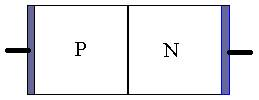
\includegraphics[width=0.3\linewidth,height=\textheight,keepaspectratio]{immagini/0.jpg}
\caption{Giunzione P-N}
\end{figure}

Nella pratica parto da un blocco puro di silicio, per poi iniettare a
\emph{strati} il drogaggio.

L'abbondanza di lacune in p è considerabile come una carenza di
elettroni, di cui n \emph{abbonda}. Ciò genera una \textbf{migrazione}
di elettroni da N verso P, detta anche \emph{corrente di diffusione}.

Tale fenomeno carica in modo \emph{positivo} n (meno elettroni), e in
modo \emph{negativo} p (più elettroni). \newline Tali cariche generano
dei campi elettrici (positivo su n e negativo su p), i quali impediscono
un ulteriore passaggio di carica, ottenendo allora un
\textbf{equilibrio}.

Nel punto di contatto si crea così una zona in cui tutte le lacune sono
state riempite, e tutti gli elettroni extra di p ceduti. Tale zona è
detta \textbf{depletion layer} (regione di svuotamento a carica
spaziale), al cui interno \textbf{non} vi sono portatori mobili (di
carica elettrica).

\begin{figure}
\centering
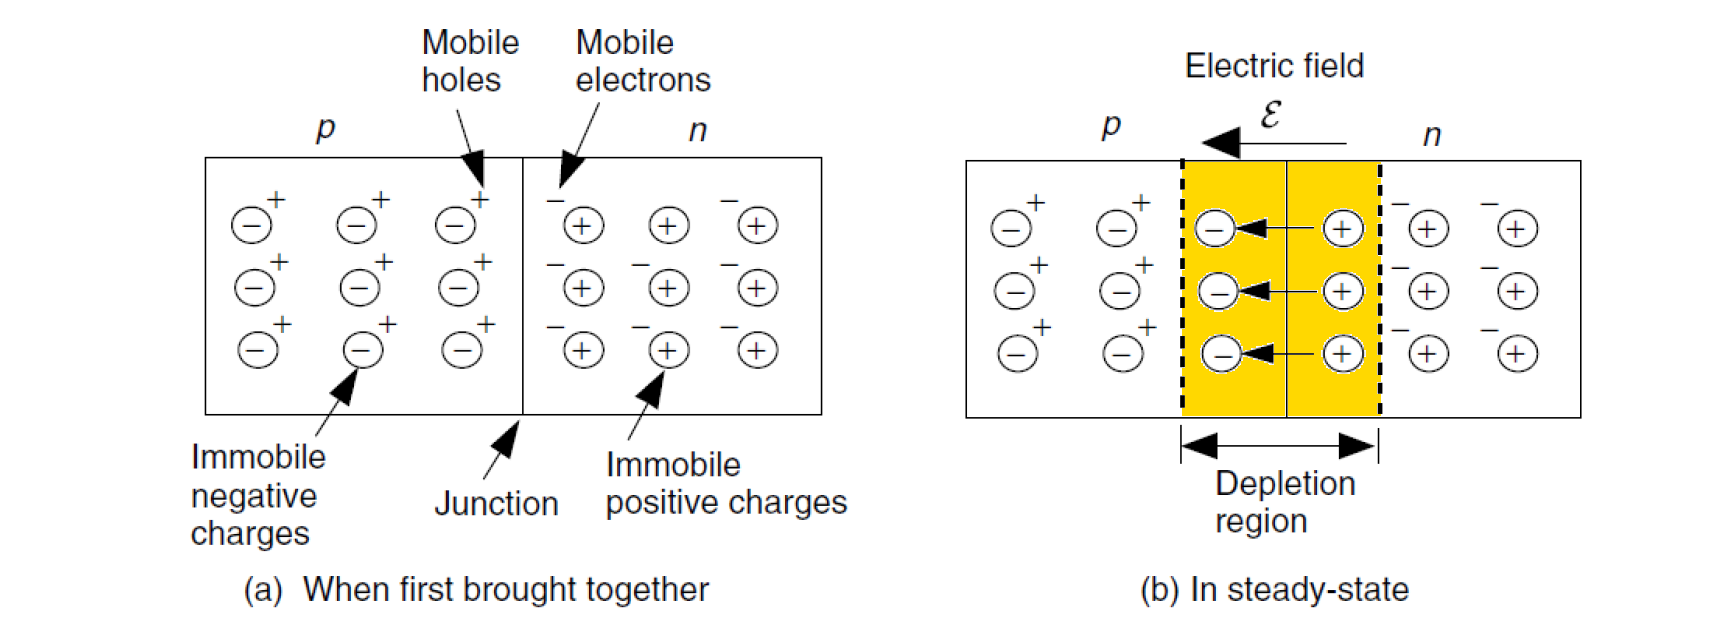
\includegraphics[width=0.68\linewidth,height=\textheight,keepaspectratio]{immagini/1.png}
\caption{Regione di svuotamento}
\end{figure}

In genere la regione di svuotamento non è simmetrica: deve valere: \[
x_P N_A = x_N N_D
\]

Come si vede nella figura 1.3 (\(x_P\) e \(x_N\) dipendono da \(N_A\) e
\(N_D\)).

\begin{itemize}
\tightlist
\item
  \(N_A > N_D \to\) più è drogata la regione più la regione di
  svuotamento è piccola.
\end{itemize}

Ricordando che il campo elettrico \(E=\int Q \,dq\), e che la tensione
(o potenziale) \(V=\int E\), si vede come il potenziale
\textbf{impedisca} il moto \colorbox{yellow}{(forse ulteriore?,
dei rimanenti elettroni)} \(p\rightarrow n\) (delle lacune) e
\(n\rightarrow p\) (degli elettroni).

\begin{figure}
\centering
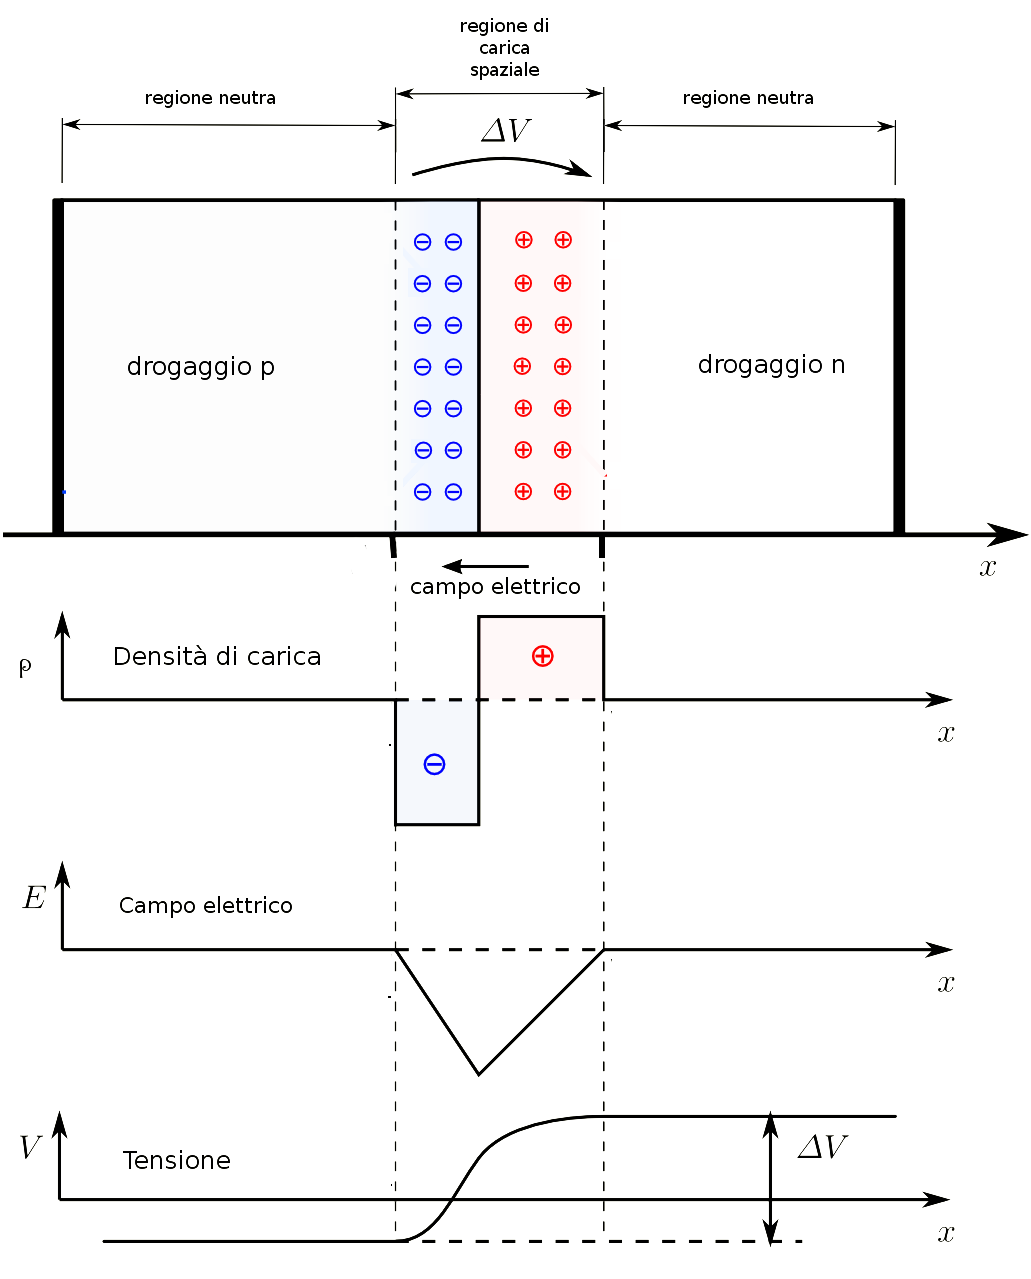
\includegraphics[width=\linewidth,height=0.35\textheight,keepaspectratio]{immagini/2.png}
\caption{``Grafici relativi alla regione di svuotamento''}
\end{figure}

\subsection{Diodo}\label{diodo}

Il simbolo circuitale della giunzione p-n, detta
\textbf{diodo}\footnote{Un diodo è un dispositivo elettrico che permette
  alla corrente di muoversi attraverso di esso in una direzione con
  molta più facilità che nell'altra. È il dispositivo più semplice che
  fa uso di una giunzione p-n.} è

\begin{center}
\begin{circuitikz}
  \draw (0,0) node[left]{A} to[diode,color=red] (2,0) node[right]{K};
\end{circuitikz}
\end{center}

dove a sinistra abbiamo un \textbf{anodo} A (dal greco \emph{salita}), e
a destra un \textbf{catodo} K (dal greco \emph{discesa}).

Sia la zone p che la zona n sono munite di un contatto elettrico (detto
\textbf{reoforo}), in modo tale che sia possibile applicarvi una
tensione. È da notare come la zona n in contatto col suo reoforo deve
essere molto drogata \colorbox{yellow}{(approfondire)}.

\subsubsection{Polarizzazione}\label{polarizzazione}

In base all'applicazione di un potenziale sul diodo posso distinguere
la:

\begin{itemize}
\tightlist
\item
  Polarizzazione \textbf{diretta} (forward bias): applico un potenziale
  positivo sull'anodo A e negativo sul catodo K, ``alzando'' il
  potenziale
\end{itemize}

\subsubsection{Diodi Speciali}\label{diodi-speciali}

\begin{center}
\begin{circuitikz}
  \draw (0,0) node[left]{+} to[diode, l_=Diodo normale] (2,0) node[right]{-};
  \draw (4,0) node[left]{-} to[diode, l_=Fotodiodo] node[right]{+} (6,0);
\end{circuitikz}
\end{center}

\appendix

\chapter{Esercizi}\label{esercizi}

\section{Esercizi capitolo 1}\label{esercizi-capitolo-1}

\chapter{}\label{section}

\section{Semiconduttori e bande}\label{semiconduttori-e-bande}

Gli elettroni in un solido allo stato fondamentale e a temperatura \(0\)
kelvin, in obbedienza alla loro natura fermionica e al principio di
Pauli che preclude ai fermioni il fatto di potersi trovare in due nello
stesso stato, riempiono gli stati elettronici loro consentiti partendo
dal livello energetico più basso via via su, fino a che tutti gli
elettroni del solido hanno trovato un'accomodazione. Si distribuiscono
cioè rispettando la distribuzione di Fermi-Dirac calcolata a temperatura
0 kelvin. Nei metalli, il livello energetico più alto occupato si
definisce livello di Fermi.

\begin{figure}
\centering
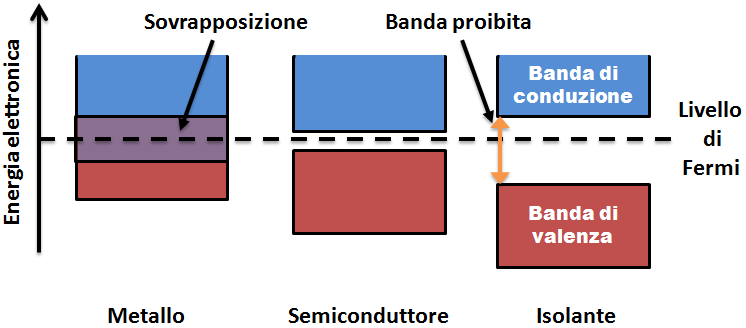
\includegraphics[width=0.5\linewidth,height=\textheight,keepaspectratio]{immagini/bande.png}
\caption{Schema semplificato della struttura elettronica a bande per
metalli, semiconduttori e isolanti.}
\end{figure}

A questo punto possono verificarsi diverse possibilità:

\begin{itemize}
\tightlist
\item
  Vi è una banda, o più di una fra le ultime riempite da elettroni, che
  è parzialmente riempita e restano degli stati vuoti. In tal caso si ha
  a che fare con un metallo, cioè un sistema in cui gli ultimi elettroni
  hanno la possibilità di spostarsi in livelli energetici molto vicini,
  infinitesimalmente più alti in energia, e dunque hanno la possibilità
  di una mobilità elevata che porta il sistema ad essere un buon
  conduttore di elettricità.
\item
  L'ultima banda è stata riempita completamente in modo tale che il
  prossimo stato elettronico consentito si trovi sulla banda successiva
  e fra questa banda e la banda completamente riempita c'è una banda
  proibita (\emph{band gap}) di energie. In tal caso il solido è un
  dielettrico.
\item
  Si parla infine di semiconduttore nel caso di un isolante in cui la
  banda proibita è talmente piccola che a temperatura ambiente c'è una
  certa probabilità che gli elettroni si trovino a saltare la banda
  proibita per agitazione termica, e dunque il sistema si trovi in una
  situazione prossima a quella di un metallo, con valori di
  conducibilità elettrica non nulli.
\end{itemize}

(N.B paragrafo proveniente da
\href{https://it.wikipedia.org/wiki/Struttura_elettronica_a_bande}{Wikipedia})

\backmatter
\end{document}
